%%%%%%%%%%%%%%%%%%%%%%%%%%%%%%%%%%%%%%%%%
% Programming/Coding Assignment
% LaTeX Template
%
% This template has been downloaded from:
% http://www.latextemplates.com
%
% Original author:
% Ted Pavlic (http://www.tedpavlic.com)
%
% Note:
% The \lipsum[#] commands throughout this template generate dummy text
% to fill the template out. These commands should all be removed when 
% writing assignment content.
%
% This template uses a Perl script as an example snippet of code, most other
% languages are also usable. Configure them in the "CODE INCLUSION 
% CONFIGURATION" section.
%
%%%%%%%%%%%%%%%%%%%%%%%%%%%%%%%%%%%%%%%%%

%----------------------------------------------------------------------------------------
%	PACKAGES AND OTHER DOCUMENT CONFIGURATIONS
%----------------------------------------------------------------------------------------

\documentclass{article}

\usepackage{fancyhdr} % Required for custom headers
\usepackage{lastpage} % Required to determine the last page for the footer
\usepackage{extramarks} % Required for headers and footers
\usepackage[usenames,dvipsnames]{color} % Required for custom colors
\usepackage{graphicx} % Required to insert images
\usepackage{listings} % Required for insertion of code
\usepackage{courier} % Required for the courier font
\usepackage{lipsum} % Used for inserting dummy 'Lorem ipsum' text into the template
\usepackage{algorithm}
\usepackage[noend]{algpseudocode}
\usepackage{amsmath}
\usepackage{amssymb}
% Margins
\topmargin=-0.45in
\evensidemargin=0in
\oddsidemargin=0in
\textwidth=6.5in
\textheight=9.0in
\headsep=0.25in

\linespread{1.1} % Line spacing

% Set up the header and footer
\pagestyle{fancy}
\lhead{\hmwkAuthorName} % Top left header
\chead{\hmwkClass\ (\hmwkClassInstructor\ \hmwkClassTime): \hmwkTitle} % Top center head
\rhead{\firstxmark} % Top right heaer
\lfoot{\lastxmark} % Bottom left footer
\cfoot{} % Bottom center footer
\rfoot{Page\ \thepage\ of\ \protect\pageref{LastPage}} % Bottom right footer
\renewcommand\headrulewidth{0.4pt} % Size of the header rule
\renewcommand\footrulewidth{0.4pt} % Size of the footer rule

\setlength\parindent{0pt} % Removes all indentation from paragraphs

%----------------------------------------------------------------------------------------
%	CODE INCLUSION CONFIGURATION
%----------------------------------------------------------------------------------------

\definecolor{MyDarkGreen}{rgb}{0.0,0.4,0.0} % This is the color used for comments
\lstloadlanguages{Perl} % Load Perl syntax for listings, for a list of other languages supported see: ftp://ftp.tex.ac.uk/tex-archive/macros/latex/contrib/listings/listings.pdf
\lstset{language=Perl, % Use Perl in this example
        frame=single, % Single frame around code
        basicstyle=\small\ttfamily, % Use small true type font
        keywordstyle=[1]\color{Blue}\bf, % Perl functions bold and blue
        keywordstyle=[2]\color{Purple}, % Perl function arguments purple
        keywordstyle=[3]\color{Blue}\underbar, % Custom functions underlined and blue
        identifierstyle=, % Nothing special about identifiers                                         
        commentstyle=\usefont{T1}{pcr}{m}{sl}\color{MyDarkGreen}\small, % Comments small dark green courier font
        stringstyle=\color{Purple}, % Strings are purple
        showstringspaces=false, % Don't put marks in string spaces
        tabsize=5, % 5 spaces per tab
        %
        % Put standard Perl functions not included in the default language here
        morekeywords={rand},
        %
        % Put Perl function parameters here
        morekeywords=[2]{on, off, interp},
        %
        % Put user defined functions here
        morekeywords=[3]{test},
       	%
        morecomment=[l][\color{Blue}]{...}, % Line continuation (...) like blue comment
        numbers=left, % Line numbers on left
        firstnumber=1, % Line numbers start with line 1
        numberstyle=\tiny\color{Blue}, % Line numbers are blue and small
        stepnumber=5 % Line numbers go in steps of 5
}

% Creates a new command to include a perl script, the first parameter is the filename of the script (without .pl), the second parameter is the caption
\newcommand{\perlscript}[2]{
\begin{itemize}
\item[]\lstinputlisting[caption=#2,label=#1]{#1.pl}
\end{itemize}
}

%----------------------------------------------------------------------------------------
%	DOCUMENT STRUCTURE COMMANDS
%	Skip this unless you know what you're doing
%----------------------------------------------------------------------------------------

% Header and footer for when a page split occurs within a problem environment
\newcommand{\enterProblemHeader}[1]{
\nobreak\extramarks{#1}{#1 continued on next page\ldots}\nobreak
\nobreak\extramarks{#1 (continued)}{#1 continued on next page\ldots}\nobreak
}

% Header and footer for when a page split occurs between problem environments
\newcommand{\exitProblemHeader}[1]{
\nobreak\extramarks{#1 (continued)}{#1 continued on next page\ldots}\nobreak
\nobreak\extramarks{#1}{}\nobreak
}

\setcounter{secnumdepth}{0} % Removes default section numbers
\newcounter{homeworkProblemCounter} % Creates a counter to keep track of the number of problems

\newcommand{\homeworkProblemName}{}
\newenvironment{homeworkProblem}[1][Problem \arabic{homeworkProblemCounter}]{ % Makes a new environment called homeworkProblem which takes 1 argument (custom name) but the default is "Problem #"
\stepcounter{homeworkProblemCounter} % Increase counter for number of problems
\renewcommand{\homeworkProblemName}{#1} % Assign \homeworkProblemName the name of the problem
\section{\homeworkProblemName} % Make a section in the document with the custom problem count
\enterProblemHeader{\homeworkProblemName} % Header and footer within the environment
}{
\exitProblemHeader{\homeworkProblemName} % Header and footer after the environment
}

\newcommand{\problemAnswer}[1]{ % Defines the problem answer command with the content as the only argument
\noindent\framebox[\columnwidth][c]{\begin{minipage}{0.98\columnwidth}#1\end{minipage}} % Makes the box around the problem answer and puts the content inside
}

\newcommand{\homeworkSectionName}{}
\newenvironment{homeworkSection}[1]{ % New environment for sections within homework problems, takes 1 argument - the name of the section
\renewcommand{\homeworkSectionName}{#1} % Assign \homeworkSectionName to the name of the section from the environment argument
\subsection{\homeworkSectionName} % Make a subsection with the custom name of the subsection
\enterProblemHeader{\homeworkProblemName\ [\homeworkSectionName]} % Header and footer within the environment
}{
\enterProblemHeader{\homeworkProblemName} % Header and footer after the environment
}

%----------------------------------------------------------------------------------------
%	NAME AND CLASS SECTION
%----------------------------------------------------------------------------------------

\newcommand{\hmwkTitle}{Mid Term} % Assignment title
\newcommand{\hmwkDueDate}{Monday,\ Nov.\ 23,\ 2015} % Due date
\newcommand{\hmwkClass}{ CAP 5638} % Course/class
\newcommand{\hmwkClassTime}{10:10am} % Class/lecture time
\newcommand{\hmwkClassInstructor}{XiuWen Liu} % Teacher/lecturer
\newcommand{\hmwkAuthorName}{Jian Wang} % Your name

%----------------------------------------------------------------------------------------
%	TITLE PAGE
%----------------------------------------------------------------------------------------

\title{
\vspace{2in}
\textmd{\textbf{\hmwkClass:\ \hmwkTitle}}\\
\normalsize\vspace{0.1in}\small{Due\ on\ \hmwkDueDate}\\
\vspace{0.1in}\large{\textit{\hmwkClassInstructor\ \hmwkClassTime}}
\vspace{3in}
}

\author{\textbf{\hmwkAuthorName}}
\date{} % Insert date here if you want it to appear below your name

%----------------------------------------------------------------------------------------

\begin{document}

\maketitle

%----------------------------------------------------------------------------------------
%	TABLE OF CONTENTS
%----------------------------------------------------------------------------------------

%\setcounter{tocdepth}{1} % Uncomment this line if you don't want subsections listed in the ToC

\newpage
\tableofcontents
\newpage

\begin{homeworkProblem}

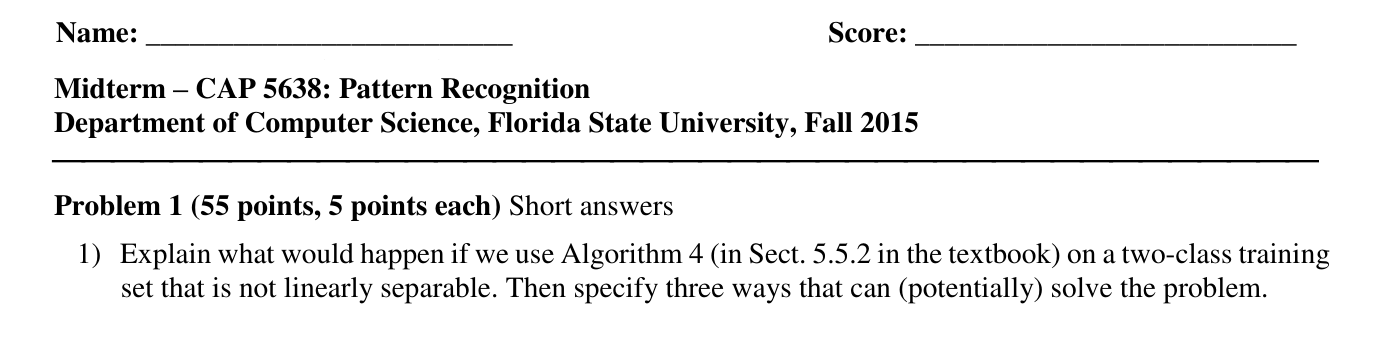
\includegraphics[width=1\columnwidth]{problem1_1.png}

Answer:\\
If the two class training set is not linearly separable, the corrections in an error-correction procedure in algorithm 4 can never cease. So Algorithm 4 will never converge and can not stop. \\

The method to solve the problem:\\
1) We can use a nonlinear mapping to make the problem separable\\
2) We can nultiple linear discriminant functions\\
3) We can learn nonlinear discriminant functions directly.\\


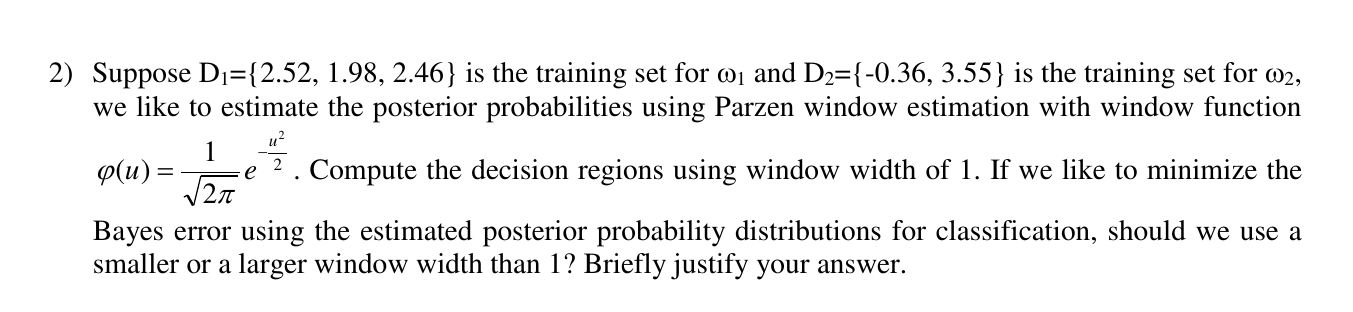
\includegraphics[width=1\columnwidth]{problem1_2.png}

Answer:\\
1) For the parzen windows, we can use the following formula to calculate the posterior probability:\\
\begin{equation*}
p_n(x)=\frac{1}{n}\sum_{i=1}^{n}\frac{1}{V_n}\varphi(\frac{x-x_i}{h_n})
\end{equation*}
where the $h_n$=1.

In this case, we can write the formula based on the dataset,given a test data $x$.\\
\begin{equation*}
p_1(x)=\frac{1}{\sqrt{2\pi}}\frac{1}{n}(e^{-\frac{({x-2.52})^2}{2}}+e^{-\frac{({x-1.98})^2}{2}}+e^{-\frac{({x-2.46})^2}{2}})
\end{equation*}

\begin{equation*}
p_2(x)=\frac{1}{\sqrt{2\pi}}\frac{1}{n}(e^{-\frac{({x+0.36})^2}{2}}+e^{-\frac{({x-3.55})^2}{2}})
\end{equation*}
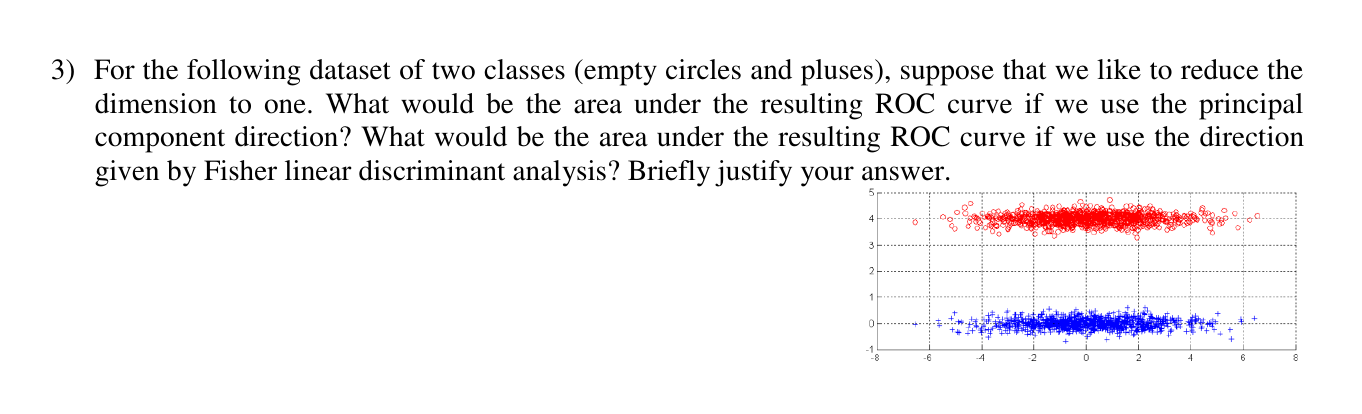
\includegraphics[width=1\columnwidth]{problem1_3.png}
The decision boundary is the $x_0$ which make $p_1(x)$ equal to the $p_2(x)$, so the decision region is that, when $x>x_0$, x belongs to class 1 and when  $x<=x_0$ x belongs to class 2


Answer:\\


PCA: : Perform dimensionality reduction while preserving as
much of the variance in the high dimensional space as
possible.
\\
FDA:Perform dimensionality reduction while preserving as
much of the class discriminatory information as possible.\\
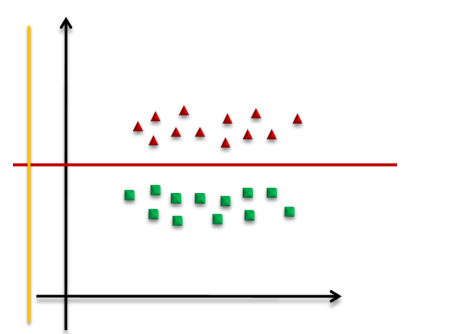
\includegraphics[scale=0.5]{reduction1.png}
In this case: we can see that the data can be classified by a horizontal line, however the principal component will be the $x_1$.

So the PCA will have higher variance and bad discriminability:\\

\includegraphics[scale=0.8]{reduction2.png}

and the FDA will have smaller variance and good  discriminability


\includegraphics[scale=0.8]{reduction3.png}

For the area under the ROC curve, the PCA will have the region under the line $y=x$, which will be around 0.5.\\

and for the FDA the area of ROC curve will be around the unit square which will be around 1.

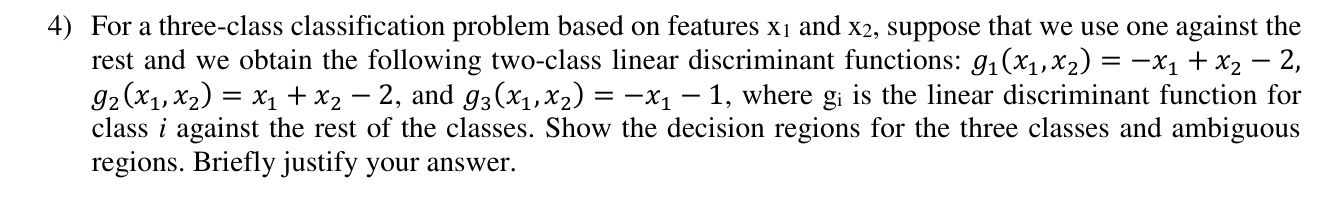
\includegraphics[width=1\columnwidth]{problem1_4.png}

Answer:\\

Use the one against all method, so if the test data is belongs to class 1, the $g_1(x)$ will be bigger than the $g_2(x)$ and $g_3(x)$. Same situation for the class 2 and class 3. 
So when test data $x$ belongs to class 1:\\
$g_1(x_1,x_2)>g_2(x_1,x_2)\Rightarrow-2x_1>0$ and $g_1(x_1,x_2)>g_3(x_1,x_2)\Rightarrow x_2>1$\\

so: $x_1<0$ and $x_2>1$\\
When test data $x$ belongs to class 1:\\
$g_2(x_1,x_2)>g_1(x_1,x_2)\Rightarrow-2x_1>0$ and $g_2(x_1,x_2)>g_3(x_1,x_2)\Rightarrow x_2>1$\\

When test data $x$ belongs to class 2:\\
$g_1(x_1,x_2)>g_2(x_1,x_2)\Rightarrow2x_1>0$ and $g_1(x_1,x_2)>g_2(x_1,x_2)\Rightarrow 2x_1+x_2-1>0$\\

so : $x_1>0$ and $x_2>-2x_1+1$\\

When test data $x$ belongs to class 3:\\
$g_3(x_1,x_2)>g_1(x_1,x_2)\Rightarrow-x_2+1>0$ and $g_3(x_1,x_2)>g_2(x_1,x_2)\Rightarrow -2x_1-x_2+1>0$\\

so : $x_1>0$ and $x_2<-2x_2+1$ 

the decision regions for the three class is as the following chart.

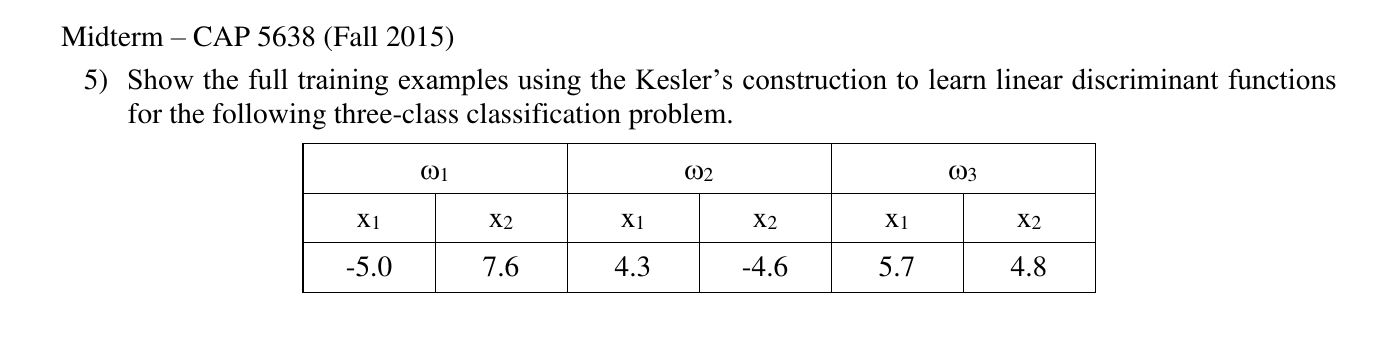
\includegraphics[width=1\columnwidth]{problem1_5.png}

Answer:\\

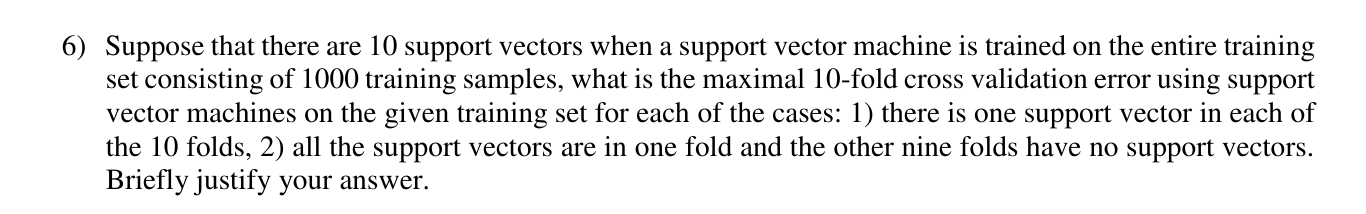
\includegraphics[width=1\columnwidth]{problem1_6.png}

Answer:\\

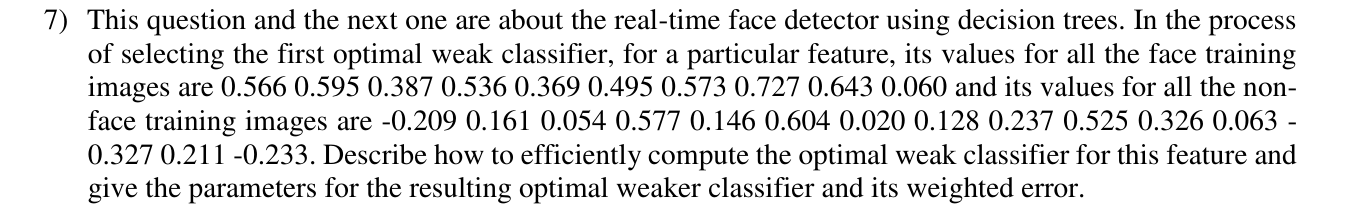
\includegraphics[width=1\columnwidth]{problem1_7.png}

Answer:\\

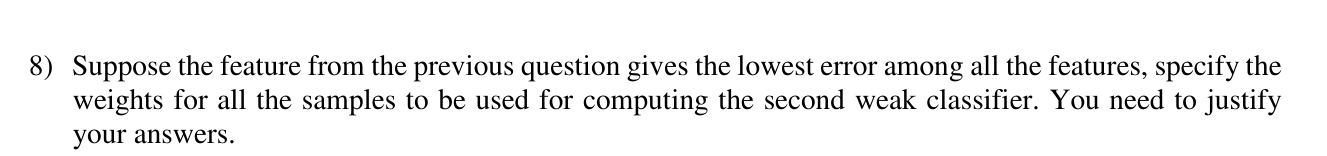
\includegraphics[width=1\columnwidth]{problem1_8.png}

Answer:\\

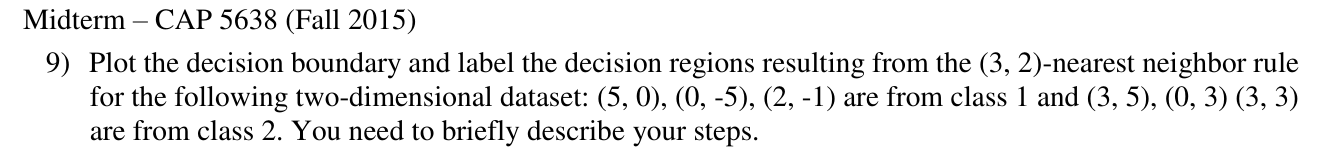
\includegraphics[width=1\columnwidth]{problem1_9.png}

Answer:\\

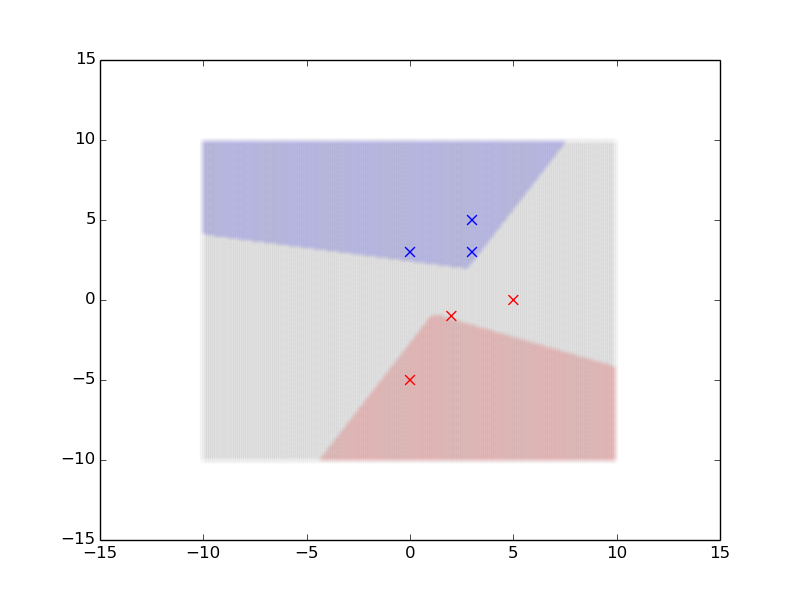
\includegraphics[width=1\columnwidth]{tree_region.png}

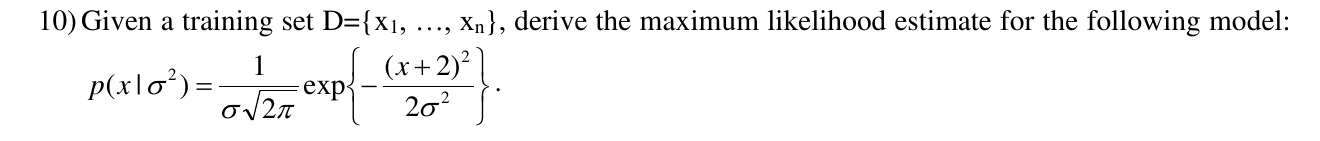
\includegraphics[width=1\columnwidth]{problem1_10.png}

Answer:\\

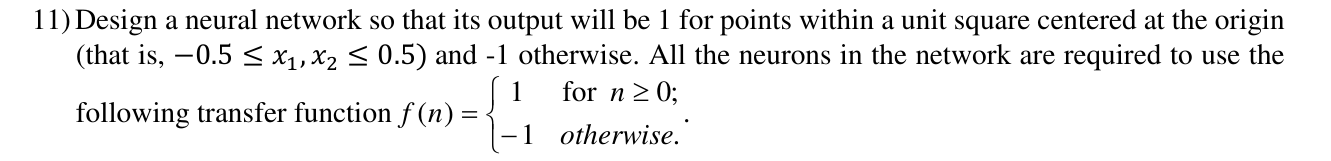
\includegraphics[width=1\columnwidth]{problem1_11.png}

Answer:\\


\end{homeworkProblem}

\begin{homeworkProblem}

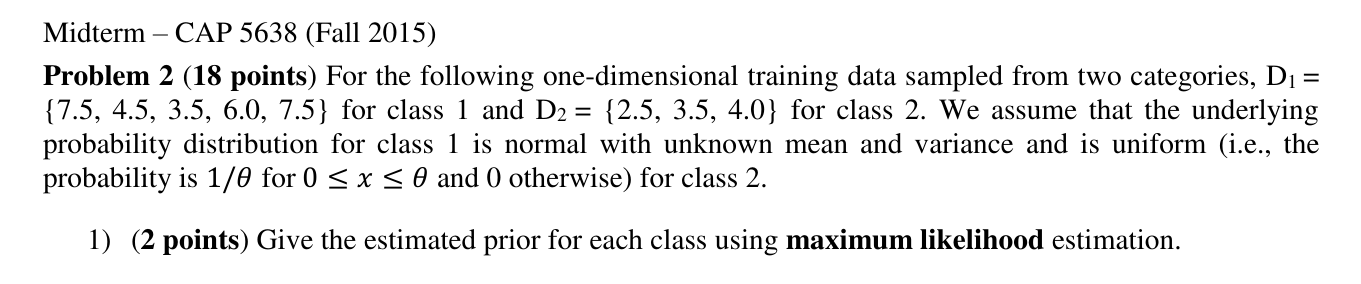
\includegraphics[width=1\columnwidth]{problem2_1.png}

Answer:\\

We denote variable $x$ as 1 if x belongs to class 1, as 0 if $x$ belongs to class 2. 

$p$ as the probability if $x =1 $. \\

so the likelihood for p given dataset{$x_i$}is:\\

\begin{equation*}
\prod_{i=1}^{n}p^{x_i}p^{1-x_i}
\end{equation*}

so the maximum likelihood of p is: \\

\begin{equation*}
p = \frac{\sum_{i=1}^{n}x_i}{n}
\end{equation*}
\end{homeworkProblem}

In this case: the prior probability that data belongs to class 1 $p = 5/8$ and the 
priror probability that data belongs to class 2 is $1-p=3/8$ 

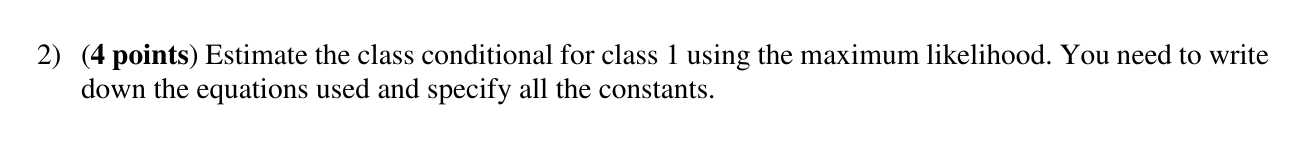
\includegraphics[width=1\columnwidth]{problem2_2.png}

Answer: \\

we know that the maximum likelihood for normal distribution is:\\ 
$\mu$ is the sample mean and the $\sigma$ is the sample standard deviation.\\
in this case: \\
\begin{equation*}
\mu= \frac{1}{5}(7.5+ 4.5+3.5+6.0 + 7.5)=5.8
\end{equation*}

\begin{equation*}
\sigma^2= \frac{1}{5}((7.5-5.8)^2+ (4.5-55.8)^2+(3.5-5.8)^2+(6.0-5.8)^2 + (7.5-5.8)^2)=2.56
\end{equation*}

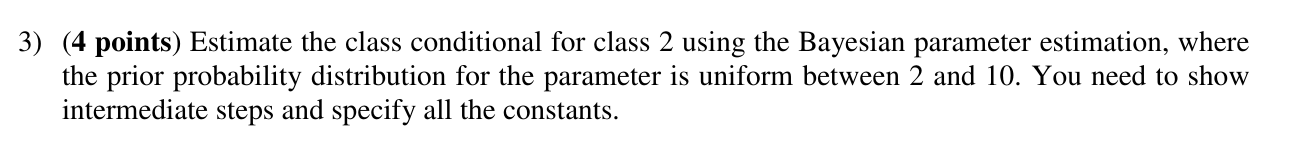
\includegraphics[width=1\columnwidth]{problem2_3.png}
Answer:\\
\begin{equation*}
p(\theta|D_0)=\left\{
\begin{aligned}
\frac{1}{8},&\quad 2\leq \theta \leq 10\\
0,&\quad otherwise
\\
\end{aligned}
\right.
\end{equation*}

\begin{equation*}
p(\theta|D_1)=\left\{
\begin{aligned}
\frac{1}{\theta}\frac{1}{(ln10-ln2.5)},&\quad 2.5\leq \theta \leq 10\\
0,&\quad otherwise
\\
\end{aligned}
\right.
\end{equation*}

\begin{equation*}
p(\theta|D_2)=\left\{
\begin{aligned}
\frac{1}{\theta^2}\frac{1}{(\frac{1}{3.5}-\frac{1}{10})},&\quad 3.5\leq \theta \leq 10\\
0,&\quad otherwise
\\
\end{aligned}
\right.
\end{equation*}



\begin{equation*}
p(\theta|D_3)=\left\{
\begin{aligned}
\frac{1}{\theta^3}\frac{2}{(\frac{1}{4.0^2}-\frac{1}{10^2})}=\frac{1}{\theta^3}{38.10},&\quad 4.0\leq \theta \leq 10\\
0,&\quad otherwise
\\
\end{aligned}
\right.
\end{equation*}

\begin{equation*}
p(x|D_3)=\int p(x|\theta)p(\theta|D_3)=\left\{
\begin{aligned}
\int_{4}^{10}\frac{1}{\theta}\frac{1}{\theta^3}\frac{1}{38.10}=\frac{1}{3}(\frac{1}{4^3}-\frac{1}{10^3}){38.10}=0.18573749999999997,&\quad 0\leq x\leq4\\
\int_{x}^{10}\frac{1}{\theta}\frac{1}{\theta^3}\frac{1}{38.10}=\frac{1}{3}(\frac{1}{x^3}-\frac{1}{10^3}){38.10},&\quad 4\leq x\leq 10\\
0,&\quad otherwise
\\
\end{aligned}
\right.
\end{equation*}
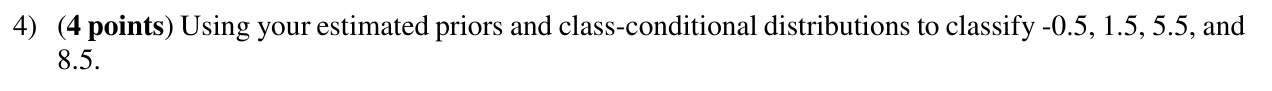
\includegraphics[width=1\columnwidth]{problem2_4.png}
Answer: \\

For the test set [-0.5,1.5,5.5,8.5], we define the discriminant function as:\\

\begin{equation*}
g_i(x)=p(x|\omega_i)p(\omega_i)
\end{equation*}

when x= -0.5: \\
$g_1(x)$=6.6994574685438983e-05, $g_2(x)$=0, so x belongs class 1\\
$g_1(x)$=0.0042100787891683278, $g_2(x)$= 0.06965156249999999, so x belongs class 2\\
$g_1(x)$=0.15312144462991092, $g_2(x)$=0.023862593914350114, so x belongs class 1\\
$g_1(x)$=0.037524023791059902, $g_2(x)$=0.0029924358843883576, so x belongs class 1\\

the final result are [1,2,1,1]

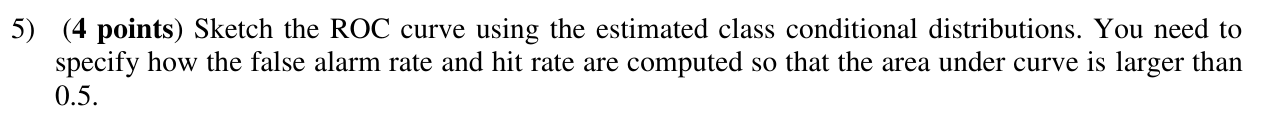
\includegraphics[width=1\columnwidth]{problem2_5.png}
Answer:\\
The following chart showed the probability density function of the two class, \\ 
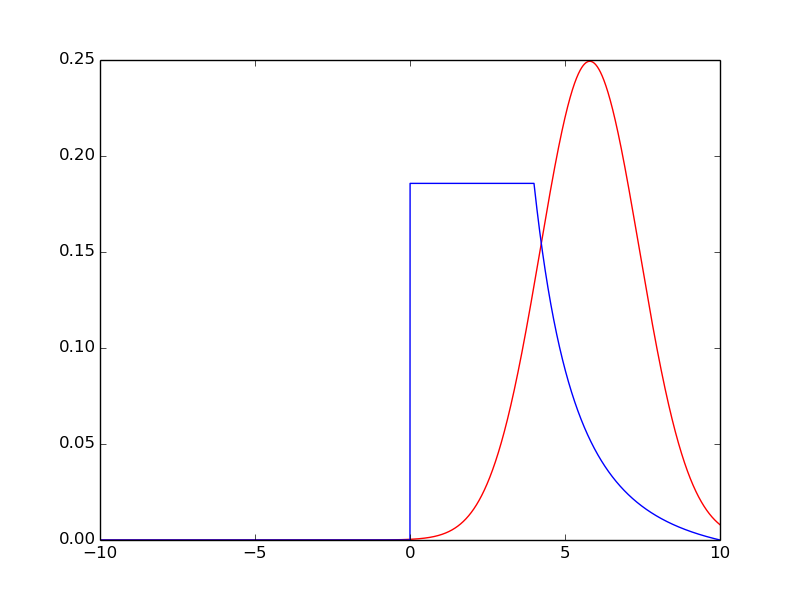
\includegraphics[scale=0.5]{roc_density.png}
Roc curve is:\\

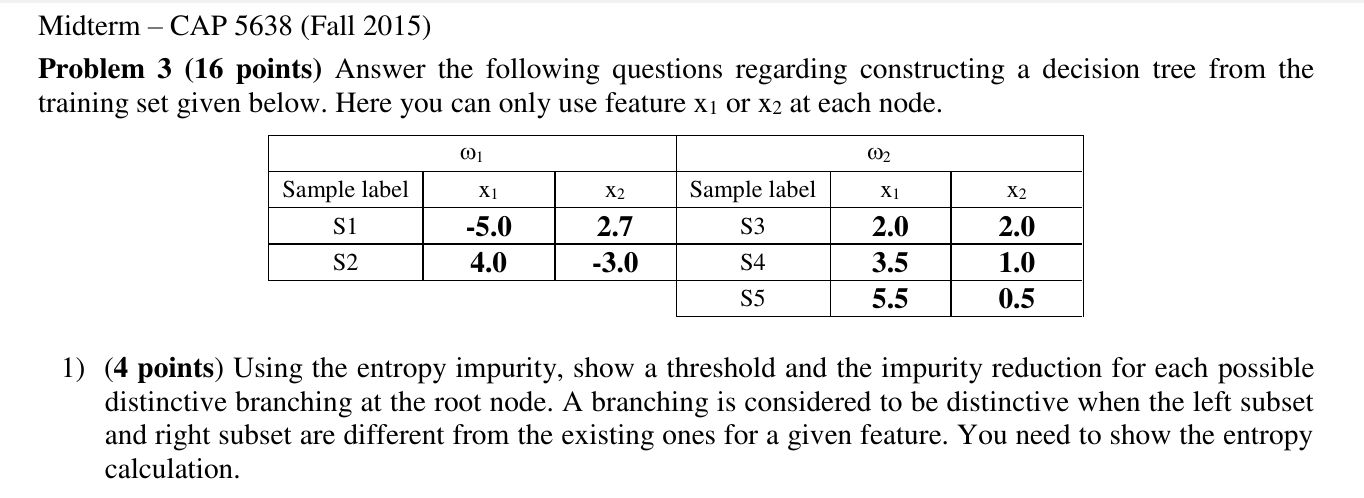
\includegraphics[width=1\columnwidth]{problem3_1.png}

Answer:\\
The data was shown on the following chart:\\

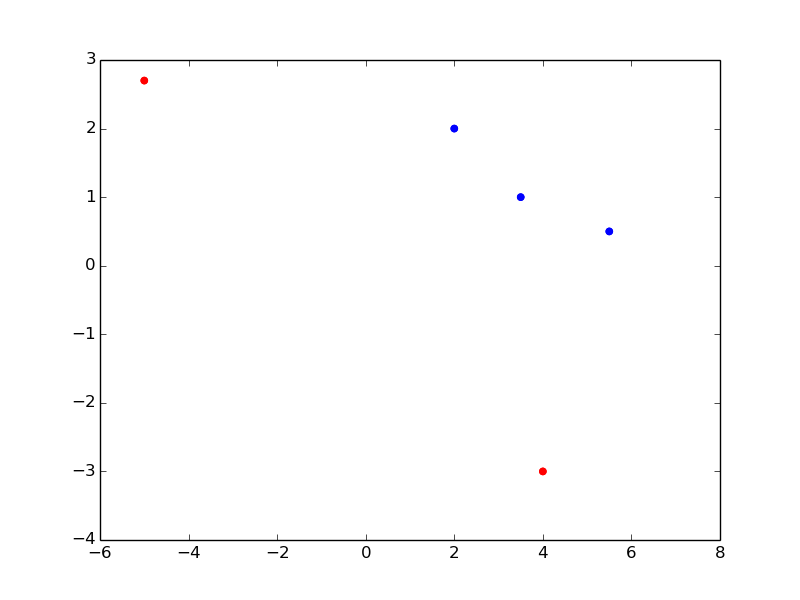
\includegraphics[width=1\columnwidth]{tree_prob.png}


first, we can calculate the original entropy:\\

\begin{equation*}
Entropy_0=-\frac{2}{5}*log_2{\frac{2}{5}}-\frac{3}{5}*log_2{\frac{3}{5}}=0.9710
\end{equation*}

next need found a root which has the biggest information gain.\\
the sorted $x_1$ value is [-5,2,3.5,4,5.5]\\
the sorted $x_2$ value is [-3,0.5,1,2,2.7]\\

calculate the mid point for each interval of $x_1$ and $x_2$,show the process in the following:\\

when $x_1<-1.5$ , on the left one node is class 2, entropy is 0, on the right, three node is class 1, one node is class 2, so the entropy will be:\\

\begin{equation*}
Entropy=-\frac{1}{4}*log_2{\frac{1}{1}}-\frac{3}{4}*log_2{\frac{3}{4}}=0.8113
\end{equation*}

so the information gain is:\\



\begin{equation*}
\Delta i(N)=i(N)-\sum_{1}^{2}p_ki(N_k)=0.9710 -\frac{4}{5}*0.8113=0.32196
\end{equation*}

for $x_1<2.75$: $\Delta i(N)=0.025$\\
for $x_1<3.75$: $\Delta i(N)=0.025$\\
for $x_1<4.75$: $\Delta i(N)=0.1710$\\
for $x_2<-1.25$: $\Delta i(N)=0.32196$\\
for $x_2<0.75$: $\Delta i(N)=0.025$\\
for $x_2<1.5$: $\Delta i(N)=0.025$\\
for $x_2<2.35$: $\Delta i(N)=0.32196$\\
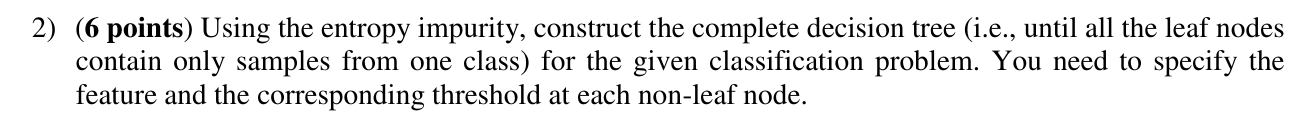
\includegraphics[width=1\columnwidth]{problem3_2.png}

Answer:\\
we can find a decision tree by: 
$x_1 < -1.5$, data belongs to class 2, and when $x_1 >-1.5$ and $x_2<-1.25$ data belongs to class 2, otherwise data belongs to class 1.\\
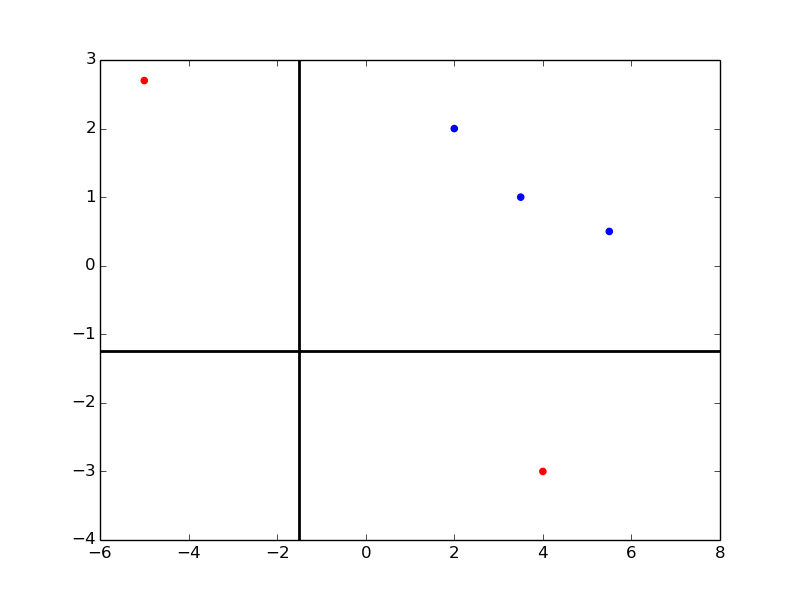
\includegraphics[scale=0.5]{tree_boundary.png}

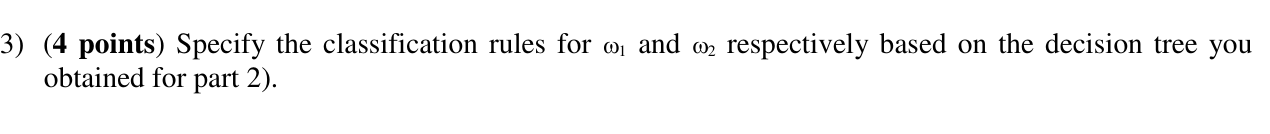
\includegraphics[width=1\columnwidth]{problem3_3.png}\\
Answer:\\

similar answer for the problem 2,
$x_1 < -1.5$, data belongs to class 2, and when $x_1 >-1.5$ and $x_2<-1.25$ data belongs to class 2, otherwise data belongs to class 1.\\
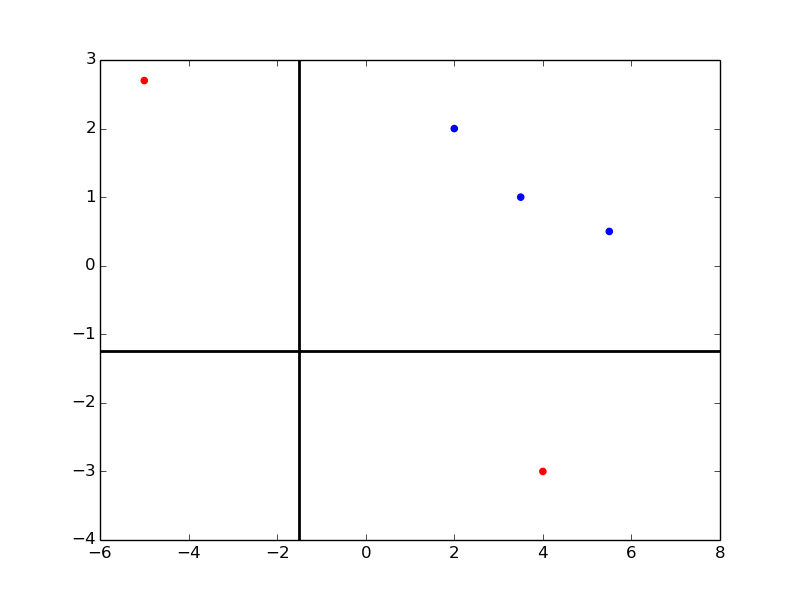
\includegraphics[scale=0.5]{tree_boundary.png}


$x_1 < -1.5$, data belongs to class 2, and when $x_1 >-1.5$ and $x_2<-1.25$ data belongs to class 2, otherwise data belongs to class 1.\\
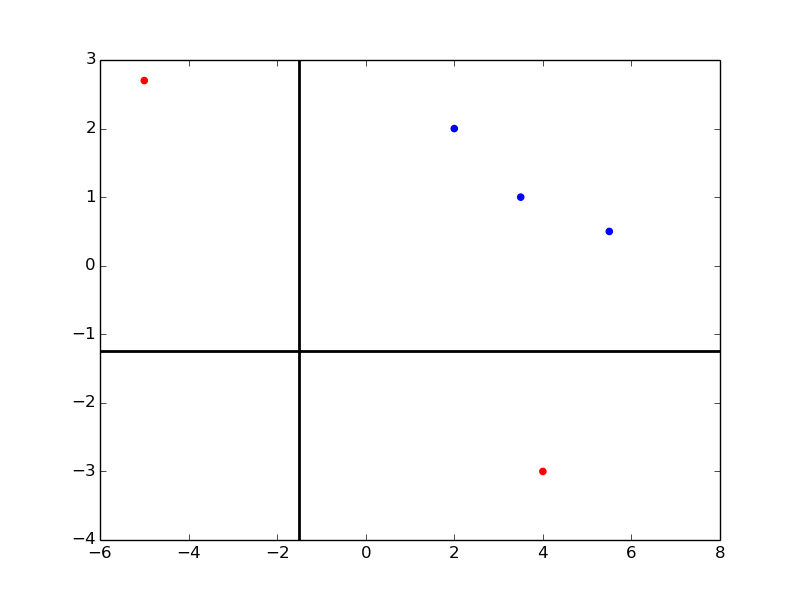
\includegraphics[scale=0.5]{tree_boundary.png}

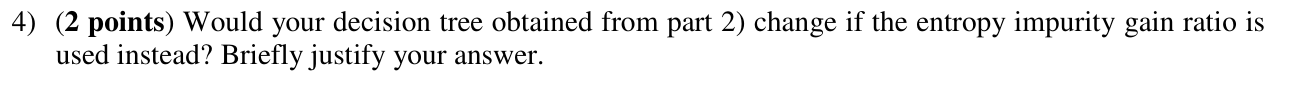
\includegraphics[width=1\columnwidth]{problem3_4.png}\\
Answer:\\
for formula for the Gain ratio is:\\
\begin{equation*}
\frac{i(N)-\sum_{k=1}^{B}P_ki(N_k)}{-\sum_{k=1}^{B}P_k log_2P_k}
\end{equation*}

For this problem, it seems no influence of for the classification of the results.

%\begin{homeworkProblem}
%Problem 1, Chapter 3 of the textbook\\
%Let $x$ have an exponential density:\\
%\begin{equation*}
%p(x|\theta)=\left\{
%\begin{aligned}
%&\theta e^{-\theta x} & & x\geq 0\\
%&0 & & otherwise
%\end{aligned}
%\right. 
%\end{equation*}
%
%(a) Plot $p(x|\theta)$ versus $x$ for $\theta=1$. Plot $p(x|\theta)$ versus $\theta$, ($0\leq \theta \leq 5)$, for $x=2$.\\
%(b) Suppose that $n$ samples $x_1,...,x_n $ are drawn independently according to $p(x|\theta)$.\\
%Show that the maximum likelihood estimate fo $\theta$ is given by:\\
%\begin{equation*}
%\hat{\theta}=\frac{1}{\frac{1}{n}\sum_{k=1}^{n} x_k}\\
%\end{equation*}
%
%Answer:\\
%(a)we draw the chart as follows, the first chart is $p(x|\theta)$ versus $x$ for $\theta=1$ and the second chart is $p(x|\theta)$ versus $\theta$, ($0\leq \theta \leq 5)$, for $x=2$\\
%
%\begin{center}
%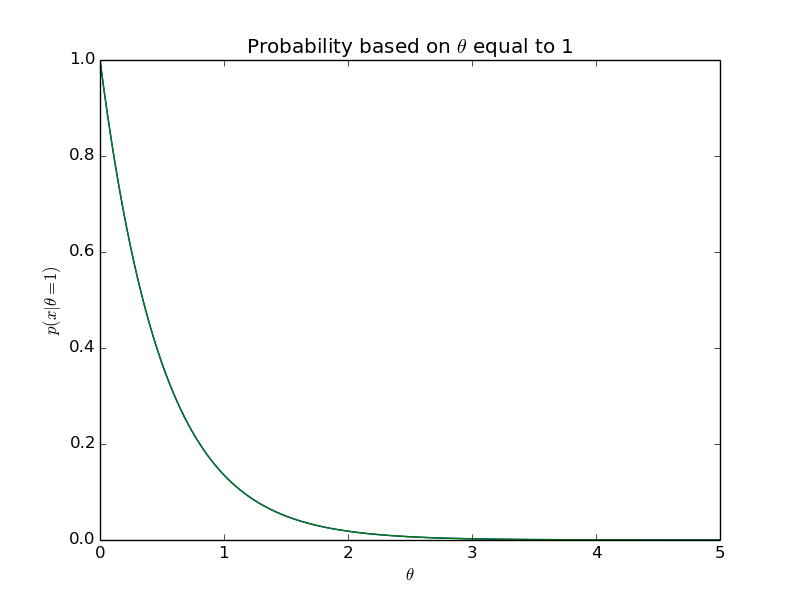
\includegraphics[width=0.75\columnwidth]{prob_theta.png}
%% Example image
%\end{center}
%
%\begin{center}
%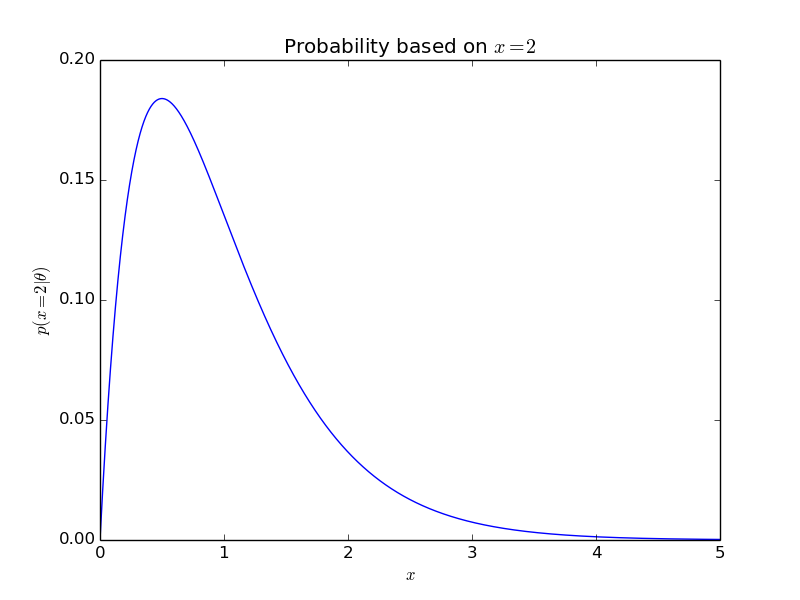
\includegraphics[width=0.75\columnwidth]{prob_x.png}
%% Example image
%\end{center}
%
%(b)The log-likelihood function is:\\
%
%\begin{equation*}
%l(\theta)= \sum_{k=1}^n ln p(x_k|\theta)=\sum_{k=1}^{n}[ln\theta-\theta x_k]=nln\theta - \theta\sum_{k=1}^{n}x_k
%\end{equation*}
%
%To find the maximum of the likelihood function, we take the first derivative of the above equation. The result is as follows:\\
%\begin{equation*}
%\begin{aligned}
%\nabla_\theta l(\theta) & =  \frac{\partial}{\partial\theta}[nln\theta-\theta\sum_{k=1}^{n}x_k]\\
%& = \frac{n}{\theta}-\sum_{k=1}^{n}x_k=0
%\end{aligned}
%\end{equation*}
%
%So the maximum -likelihood solution is:\\
%\begin{equation*}
%\hat{\theta}=\frac{1}{\frac{1}{n}\sum_{k=1}^{n}x_k}.
%\end{equation*}
%
%\end{homeworkProblem}
%
%\begin{homeworkProblem}
%Problem 3, Chapter 3 of the textbook.\\
%Maximum likelihood methods apply to estimates of prior probabilities as well. Let samples be drawn by successive, independent selections of a state of nature $\omega_i$, with unknown probability $P(\omega_i)$. Let $z_{ik}=1$ , if the state of nature for the $kth$ sample is $\omega_i$ and $z_{ik}=0$ otherwise.\\
%
%(a) Show that \\
%
%\begin{equation*}
%P(z_{i1},...,z_{in}|P(\omega_i))=\prod_{k=1}^{n} P(\omega_i)^{z_{ik}}(1-P(\omega_i))^{1-z_{ik}}
%\end{equation*}
%
%
%(b) Show that the maximum likelihood estimate for $P(\omega_i)$ is\\
%
%\begin{equation*}
%\hat{P}(\omega_i)=\frac{1}{n}\sum_{k=1}^{n}z_{ik}.
%\end{equation*}
%Interpret your result in words.\\
%
%Answer:\\
%
%We denote that \\
%\begin{equation*}
%z_{ik}=\left\{
%\begin{aligned}
%&1 & & if\ the\ state\ of\ nature\ for\ the\ k^{th}\ sample\ is\ \omega_i\\
%& 0 & & otherwise
%\end{aligned}
%\right.
%\end{equation*}
%
%(a) The sample are drawn by successive independently selection of a state of nature $\omega_i$ with probability $P(\omega_i)$. We have then :\\
%\begin{equation*}
%Pr[z_{ik}=1|P(\omega_i)]=P(\omega_i)
%\end{equation*}
%
%and:\\
%\begin{equation*}
%Pr[z_{ik}=0|P(\omega_i)]=1-P(\omega_i)
%\end{equation*}
%we can rewrite the above equation as:\\
%
%\begin{equation*}
%Pr[z_{ik}|P(\omega_i)]=[P(\omega_i)]^{z_{ik}}[1-P(\omega_i)]^{1-z_{ik}}
%\end{equation*}
%By the independence of the successive selections, we have :\\
%\begin{eqnarray*}
%P(z_{i1},...,z_{in}|P(\omega_i)) & =&\prod_{k=1}^{n}P(z_{ik}|P(\omega_i))\\
%&=& \prod_{k=1}^{n}[P(\omega_i)]^{z_{ik}}[1-P(\omega_i)]^{1-z_{ik}}
%\end {eqnarray*}
%
%(b) The log-likelihood as a function of $P(\omega_i)$ is:\\
%\begin{eqnarray*}
%l(P(\omega_i)) &=&  lnP(z_{i1},...,z_{in}|P(\omega_i))\\
%&=& ln[\prod_{k=1}^{n}[P(\omega_i)]^{z_{ik}}[1-P(\omega_i)]^{(1-z_{ik})}]\\
%&=& \sum_{k=1}^n [z_{ik}lnP(\omega_i)+(1-z_{ik})ln(1-P(\omega_i))]
%\end{eqnarray*}
%Therefore, the maximum-likelihood values for the $P(\omega_i)$ must satisfy:\\
%\begin{equation*}
%\nabla _{P(\omega_i)}l(P(\omega_i))=\frac{1}{P(\omega_i)}\sum_{k=1}^{n}z_{ik}-\frac{1}{1-P(\omega_i)}\sum_{k=1}^n(1-z_{ik})=0
%\end{equation*}
%We solve this equation and find :
%
%\begin{equation*}
%(1-\hat{P}(\omega_i))\sum_{k=1}^n z_{ik}= \hat{P}(\omega_i)\sum_{k=1}^n (1-z_{ik})
%\end{equation*}
%
%which can be rewritten as:\\
%\begin{equation*}
%\sum_{k=1}^nz_{ik}= \hat{P}(\omega_i)\sum_{k=1}^n z_{ik} + n \hat{P}(\omega_i)-\hat{P}(\omega_i)\sum_{k=1}^n z_{ik}
%\end{equation*}
%
%So the final solution is then:\\
%\begin{equation*}
%\hat{P}(\omega_i)=\frac{1}{n}\sum_{k=1}^n z_{ik}
%\end{equation*}
%
%That is, the estimate of the probability of category $\omega_i$ is merely the probability of obtaining its indicatory value in the training data,  just as we would expected.
%
%\end{homeworkProblem}
%
%\begin{homeworkProblem}
%Problem 7 , Chapter 3 od the textbook\\
%Show that if our model is poor, the maximum likelihood classifier we derive is not the best
%\textendash even among our (poor) model set \textendash by exploring the following example. Suppose we have two equally probable categories (i.e., p($\omega_1$)=P($\omega_2$)=0.5). Further, we know that $p(x|\omega_1)\sim N(0,1)$ but \textit{assume} that $p(x|\omega_2)\sim N(\mu,1)$. (That is, the parameter $\theta$ we seek by maximum likelihood techniques is the mean of the second distribution.) Image however that the \textit{true} underlying distribution is $p(x|\omega_2)\sim N(1,10^6)$.\\
%(a)what is the value of our maximum likelihood estimate $\mu$, in our poor model, given a large amount of data.\\
%(b)  What is the decision boundary arising from this maximum likelihood estimate in the poor model.\\ 
%(c) Ignore for the moment the maximum likelihood approach, and use the methods from chapter 7 to derive the Bayes optimal decision boundary given the \textit{true} underlying distributions \textendash $p(x|\omega_1) \sim N(0,1)$ and $p(x|\omega_2) \sim N(1,10^6)$. be careful to include all portions pf the decision boundary. \\
%(d) Now consider again classifiers based on the (poor) model assumption of $p(x|\omega_2) \sim N(\mu,1 ).$ Using your result immediately above, find a \textit{new} value of $\mu$ that will give lower error than the maximum likelihood classifier. \\
%(e) Discuss these results, with particular attention to the role of knowledge of the underlying model.\\
%Answer:\\
%
%
%\end{homeworkProblem}
%
%\begin{homeworkProblem}
%problem 10, Chapter 3 of the textbook (hint think about the bias and variance.)
%Suppose we employ a novel method for estimating the mean of a data set, $\mathcal{D}={x_1,x_2,...,x_n}$ : we assign the mean to the value of the first point in the set, i.e., $x_1$.\\
%(a) Show that tis method is unbiased. \\
%(b) State why this method is nevertheless highly undesirable.\\
%
%Anwser:\\
%(a)Consider the novel method of estimating the mean of a set of points as taking its first value, which we denote $M= x_1$,\\
%(a) If the expected value of a statistics is equal to the true value, then we call the statistics unbiased. for this case, if we repeat the selection of the first point of a data set we have:\\
%
%\begin{equation*}
%bias = E(M) -\mu=lim_{K\rightarrow\infty}\frac{1}{K}\sum_{k=1}^{K} M(k)-\mu=0; 
%\end{equation*}
%
%Where $M(k)$ is the first point in data set k drawn from the given distribution.\\
%
%(b) While the unusual method for estimating the mean may indeed be biased, it will generally have large variance, and this is an undesirable property. Note that $E[(x_i)-\mu)^2]=\sigma^2$, and the RMS error, $\sigma$, is independent of n.  This undesirable behavior is quite different from that of the measurement of:\\
%\begin{equation*}
%\bar{x} =\frac{1}{n}\sum_{i =1}{n}x_i
%\end{equation*}
%
%where we see:\\
%
%\begin{eqnarray*}
%E[(\bar{x}-\mu)^2] &=& E[(\frac{1}{n}\sum_{i=1}^{n}x_i-\mu)^2]\\
%&=& \frac{1}{n^2}\sum_{i=1}^{n} [E[(x_i-\mu)^2]\\
%&=& \frac{\sigma^2}{n}
%\end{eqnarray*}
%
%Thus the RMS error, $\sigma/\sqrt{n}$, approaches 0 as $1/\sqrt{n}$. Note that there are many superior method for estimating the mean, for instance the sample mean and some other re-sampling method such as "bootstrap" method. 
%
%\end{homeworkProblem}
%
%\begin{homeworkProblem}
%Suppose that the prior distribution of $\theta$ and the parametric form (a uniform distribution) remain the same as in the example given in section 3.5 in the textbook, compute first the Bayesian estimation of $\theta$ and then the estimated class conditional $p(x|D)$ for $D=\{3,9,7\}$. You need to specify the Bayesian estimation and the class conditional fully (i.e., you need to specify the functions with all required constants). Then plot the class conditional form from 0 to 10.\\
%
%Answer:\\
%
%From the example of the textbook, we know that the prior distribution of $\theta$ is a uniform distribution, which listed in the following:\\
%
%\begin{equation*}
%p(x|\theta)\sim U(0, \theta)=\left\{
%\begin{aligned}
%& 1/ \theta & & 0 \leq x \leq 10\\
%& 0 & & otherwise,  \\
%\end{aligned}
%\right.
%\end {equation*}
%
%Similarly with the example in the textbook, we will sue recursive Bayes methods to estimate $\theta$ and the underlying distribution. Before any data arrive, we have $\pagebreak(\theta|\mathcal{D}^0)=p(\theta)=U(0,10)$
%when our first data point $x_1$=3 arrives, we use the equation 54, from the textbook, to get an improved estimate:\\
%\begin{equation*}
%p(\theta|\mathcal{D}^1) \propto p(x|\theta)p(\theta|\mathcal{D}^0)=\left\{
%\begin{aligned}
%& 1/ \theta & & 3 \leq x \leq 10\\
%& 0 & & otherwise,  \\
%\end{aligned}
%\right.
%\end {equation*}
%When the next data point $ x_2 = 9 $ arrives, we have :\\
%\begin{equation*}
%p(\theta|\mathcal{D}^2) \propto p(x|\theta)p(\theta|\mathcal{D}^1)=\left\{
%\begin{aligned}
%& 1/ \theta^2 & & 9 \leq x \leq \theta\\
%& 0 & & otherwise,  \\
%\end{aligned}
%\right.
%\end {equation*}
%
%when the third data point, which is equal to 7, comes, we have:\\
%
%\begin{equation*}
%p(\theta|\mathcal{D}^3) \propto p(x|\theta)p(\theta|\mathcal{D}^2)=\left\{
%\begin{aligned}
%& 1/ \theta^3 & & 9 \leq x \leq 10\\
%& 0 & & otherwise,  \\
%\end{aligned}
%\right.
%\end {equation*}
% 
%
%The general form of the solution is:\\
%\begin{center}
%$p(\theta|\mathcal{D}^n)\propto 1/\theta^n$ for $\max_x[\mathcal{D}^n]\leq \theta\leq 10$.  
%\end{center}
%
%
%To make the above equation become the density function, we also calculate the constant term in all the $p(\theta|\mathcal{D}_i)$, which listed as follows:\\
%
%\begin{equation*}
%p(\theta|\mathcal{D}^1) =\left\{
%\begin{aligned}
%& 1/(ln(10)-ln(3)*1/ \theta & & 9 \leq x \leq 10\\
%& 0 & & otherwise,  \\
%\end{aligned}
%\right.
%\end {equation*}
%
%\begin{equation*}
%p(\theta|\mathcal{D}^2) =\left\{
%\begin{aligned}
%& 1/(1/9-1/10)*1/ \theta^2 & & 9 \leq x \leq 10\\
%& 0 & & otherwise,  \\
%\end{aligned}
%\right.
%\end {equation*}
%
%\begin{equation*}
%p(\theta|\mathcal{D}^3) =\left\{
%\begin{aligned}
%& 1/(1/162-1/200)*1/ \theta^3 & & 9 \leq x \leq 10\\
%& 0 & & otherwise,  \\
%\end{aligned}
%\right.
%\end {equation*}
%We also plot the result for the $p(\theta|\mathcal{D}^i)$ under 4 cases as follows:\\
%
%\begin{center}
%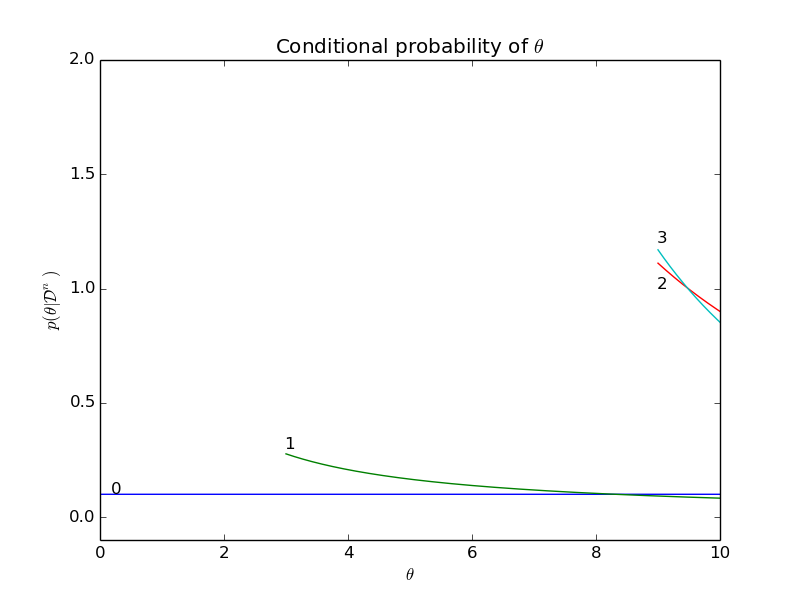
\includegraphics[width=0.75\columnwidth]{conditional_prob_theta.png} % Example image
%\end{center}
%
%next part we try to solve the conditional class probability, $p(x|\mathcal{D}^3)$, given the equation 50 on the text book, we need to solve the integration of the following equation:\\
%\begin{equation*}
%p(x|\mathcal{D})= \int p(x|\theta)p(\theta|\mathcal{D})d\theta 
%\end{equation*}
%note that $\theta$ should be bigger than x and the domain of $\theta$ is 9 to 10 in our case, so in the domain from 0 to 9 of x, the integral region of $\theta$ is 9 to 10, when x bigger than 9, the integral region of $\theta$  becomes x to 10. This means that when x is from 0 to 9, it follows an uniform distribution, and when x is bigger than 9, it follows some polynomial density function. \\ 
%Now we calculate the integration under two situation:\\
%When x is less than 9:\\
%
%\begin{equation*}
%p(x|\mathcal{D})= \int p(x|\theta)p(\theta|\mathcal{D})d\theta =\int_9^{10}
%1/(1/162-1/200)*1/ \theta^4 d\theta=0.10565302144249514
%\end{equation*}
%
%when x is bigger than 9:\\
%
%\begin{equation*}
%p(x|\mathcal{D})= \int p(x|\theta)p(\theta|\mathcal{D})d\theta =\int_x^{10}
%1/(1/162-1/200)*1/ \theta^4 d\theta=1/(1/162-1/200)*1/3*(1/x^3-1/1000)
%\end{equation*}
%
%The following chart shows the result of the conditional class probability in the domain for $x$ from 0 to 10.\\
%
%\begin{center}
%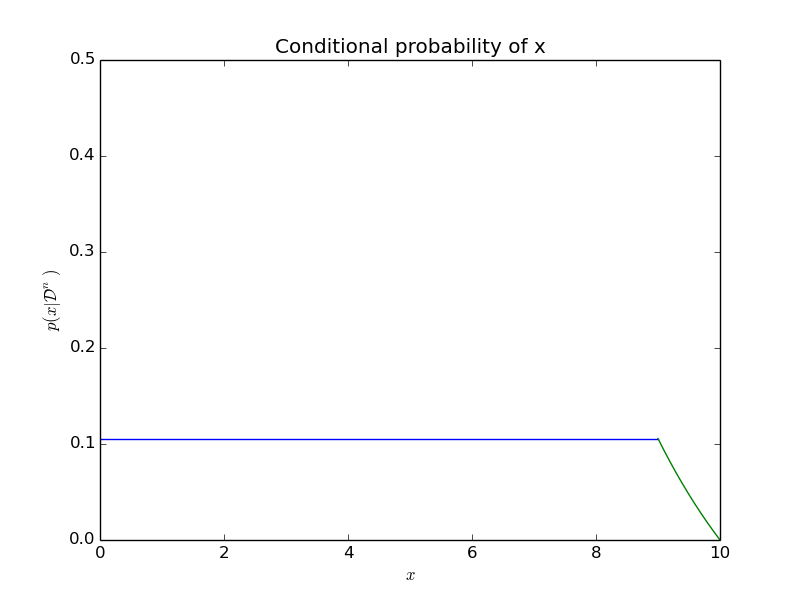
\includegraphics[width=0.75\columnwidth]{conditional_prob_xx.png} % Example image
%\end{center}
%
%\end{homeworkProblem}
%
%\begin{homeworkProblem}
%Problem 11 chapter 3 of the textbook; you only need to show the univariate case.\\
%One measure of the difference between two distribution in the same space is the \textit{Kullback-l=Leibler divergence} of Kullback-Leibler" distance":\\
%\begin{equation*}
%D_{KL}(p_1(x),p_2(x)) = \int {p_1(x)ln\frac{p_1(x)}{p_2(x)}dx}
%\end{equation*}
%( This "distance," does not obey the requisite symmetry and triangle inequalities for a metric.) Suppose we seek to approximate an arbitrary distribution $p_2(x)$ by a normal $p_1(x) \sim N(\mu, \Sigma)$. Show that the values that lead to the smallest Kullback-leibler divergence are the obvious ones:\\
%\begin{equation*}
%\begin{aligned}
%&\mu &=& \mathcal{E}_2[x]\\
%&\Sigma &=& \mathcal{E}_2[(x-\mu)(x-\mu)^t]
%\end{aligned}
%\end{equation*}
%where the expectation taken is over the density $p_(x)$.
%\end{homeworkProblem}

%
%%----------------------------------------------------------------------------------------
%%Algorithm test 
%%----------------------------------------------------------------------------------------
%\begin{homeworkProblem}
%\begin{algorithm}
%\caption{Euclid’s algorithm}\label{alg:euclid}
%\begin{algorithmic}[1]
%\Procedure{Euclid}{$a,b$}\Comment{The g.c.d. of a and b}
%\State $r\gets a\bmod b$
%\While{$r\not=0$}\Comment{We have the answer if r is 0}
%\State $a\gets b$
%\State $b\gets r$
%\State $r\gets a\bmod b$
%\EndWhile\label{euclidendwhile}
%\State \textbf{return} $b$\Comment{The gcd is b}
%\EndProcedure
%\end{algorithmic}
%\end{algorithm}
%\end{homeworkProblem}
%
%
%%----------------------------------------------------------------------------------------
%%	PROBLEM 1
%%----------------------------------------------------------------------------------------
%
%% To have just one problem per page, simply put a \clearpage after each problem
%
%
%\begin{homeworkProblem}
%Listing \ref{homework_example} shows a Perl script.
%
%\perlscript{homework_example}{Sample Perl Script With Highlighting}
%
%\lipsum[1]
%\end{homeworkProblem}
%
%%----------------------------------------------------------------------------------------
%%	PROBLEM 2
%%----------------------------------------------------------------------------------------
%
%\begin{homeworkProblem}
%\lipsum[2]
%
%\problemAnswer{
%\begin{center}
%\includegraphics[width=0.75\columnwidth]{example_figure} % Example image
%\end{center}
%
%\lipsum[3-5]
%}
%\end{homeworkProblem}
%
%%----------------------------------------------------------------------------------------

\end{document}